\documentclass{article}

\usepackage{geometry}
\usepackage{makecell}
\usepackage{array}
\usepackage{multicol}
\usepackage{setspace}
\usepackage{xcolor}
\usepackage{changepage}
\usepackage{booktabs}
\usepackage{hyperref}
\usepackage{amssymb}
\usepackage[explicit]{titlesec}
\usepackage{amsmath}
\usepackage{wrapfig}
\usepackage{graphicx}
\usepackage{titlesec}
\usepackage{float}
\newcolumntype{?}{!{\vrule width 1pt}}
\renewcommand{\contentsname}{Inhaltsverzeichnis:}
\renewcommand\theadalign{tl}
\newcommand{\paragraphlb}[1]{\paragraph{#1}\mbox{}\\}
\def\ojoin{\setbox0=\hbox{$\bowtie$}%
  \rule[-.02ex]{.25em}{.4pt}\llap{\rule[\ht0]{.25em}{.4pt}}}
\def\lojoin{\mathbin{\ojoin\mkern-5.8mu\bowtie}}
\def\rojoin{\mathbin{\bowtie\mkern-5.8mu\ojoin}}
\def\fojoin{\mathbin{\ojoin\mkern-5.8mu\bowtie\mkern-5.8mu\ojoin}}
\newcommand{\ajoin}{\ensuremath{\triangleright}}
\newcommand{\sjoin}{\ensuremath{\ltimes}}

\titleformat{\section}
  {\normalfont\Large\bfseries}{\thesection}{1em}{\hyperlink{sec-\thesection}{#1}
\addtocontents{toc}{\protect\hypertarget{sec-\thesection}{}}}
\titleformat{name=\section,numberless}
  {\normalfont\Large\bfseries}{}{0pt}{#1}

\titleformat{\subsection}
  {\normalfont\large\bfseries}{\thesubsection}{1em}{\hyperlink{subsec-\thesubsection}{#1}
\addtocontents{toc}{\protect\hypertarget{subsec-\thesubsection}{}}}
\titleformat{name=\subsection,numberless}
  {\normalfont\large\bfseries}{\thesubsection}{0pt}{#1}

\hypersetup{
    colorlinks,
    citecolor=black,
    filecolor=black,
    linkcolor=black,
    urlcolor=black
}
\setstretch{1.10}
\setlength{\parindent}{0pt}
\titlespacing\section{0pt}{12pt plus 4pt minus 2pt}{0pt plus 2pt minus 2pt}

\geometry{top=12mm, left=1cm, right=2cm}
\title{\vspace{-1cm}Relationale Datenbanken 1}
\author{Andreas Hofer}

\begin{document}
	\maketitle
	\tableofcontents
	\newpage
	\section{DB Entwurfsprozess}
	\subsection{Anforderungsanalyse}
	Der Entwurf einer Datenbank beginnt mit der Anforderungsanalyse (Requirements Engineering), in welchem man die grundlegenden Voraussetzungen festlegt. 40\% aller Projekte, welche über das Budget laufen oder scheitern, hatten eine unzureichende Anforderungsanalyse. \\
	Probleme, welche bereits in der Anforderungsanalyse erkannt werden, führen zu einer drastis
	\subsection{Funktionale/Konzeptuelle Anforderungen}
	Danach werden Anforderungen eingearbeitet. Dabei wird zwischen Konzeptionelle und Funktionale Anforderungen unterschieden. \\
	Konzeptionelle Anforderungen sind rechtliche Vorgaben. Zum Beispiel dürfen nur Daten abgefragt werden, welche auch für das Programm relevant sind. \\
	Funktionale Anforderungen hingegen sind die Vorgaben für die Verwendung des Programms. Wenn man ein rotes Kreuz in der Ecke klickt, muss sich das Fenster schließen.
	\subsection{Spezifikation von Transaktionen}
	Nach der Festlegung der Funktionalen Vorraussetzungen, werden die Transaktionen spzifiziert, welche Calls sind nötig?
	\subsection{Entity-Relationship Modell}
	Das ER-Modell beschreibt ein konzeptionelles Datenmodell und wird in einem iterativen Prozess erstellt. \\
	Im ER-Modell gibt es Entitäten, welche spezifische Objekte sind. Jedes dieser Entitäten hat spezifische Attribute. Abhängig von der Entität können diese unterschiedlich sein. Ein Tisch hat zum Beispiel die Attribute wie viele Beine er hat, welche Farbe(n) er hat und so weiter. Danach werden diese Entitäten mit ihren Attributen mit anderen Entitäten in Beziehungen gestellt (Die Relationship). \\
	Da der Prozess schrittweise geschieht, beginnt man nicht sofort mit zum Beispiel dem Datentyp einer Entität sondern beginnt zuerst sehr allgemein und wird danach immer spezifischer. \\
	Das ER-Modell ist in seiner Umsetzung sehr ähnlich der UML (Unified Modelling Language). Gleich wie die UML ist sie jedoch auch nur einen DDL und keine DML, da man zwar beschreiben kann, wie etwas umgesetzt werden sollte, die Umsetzung selbst jedoch z.B. in SQL machen muss. ER ist auch so allgemein wie möglich definiert, da es unabhängig von der letzten Umsetzung modelliert werden sollte und die endgültige Wahl der DML keine Auswirkung auf ER haben sollte. \\
	Bei der Datenmodellierung gibt es eine Vielzahl an Tools um die Datenmodellierung einfacher zu machen. \\
	Vorteil von solcher Software ist, dass man die Analyse einfach dokumentieren kann, da die Schritte genau nachvollziehbar sind und, dass Systeme schnell modelliert werden können. Jedoch werden komplexe Systeme sehr schnell unübersichtlich. \\
	In ER sind Entitäten spezifische Objekte. Die Attribute der Objekte haben jeweils einen Wert. (Key-Value-Pair) Jedes Attribut muss dabei eine Domäne besitzen (Data Type). Jedes Attribut kann nur eine Domäne besitzen und schränkt ein, was in ihr gespeichert werden kann. Spezifische Datentypen sind: \\
	\begin{itemize}
		\item{Primitive Attribute}
		\begin{itemize}
			\item{Attribute, welche aus nur einem Wert bestehen und von einem System meist nativ unterstützt wird.}
		\end{itemize}
		\item{Zusammengesetzte Attribute}
		\begin{itemize}
			\item{Attribute, welche aus mehreren primitiven Attributen zusammengesetzt wird. Zum Beispiel benötigt eine Adresse die Straße (Varchar), die Hausnummer (Integer), PLZ (AT Integer).}
		\end{itemize}
		\item{Mehrwertige Attribute}
		\begin{itemize}
			\item{Attribute, welche aus mehreren Attributen bestehen. Zum Beispiel hat jemand drei Telefonnummern und diese sollten nicht separat gespeichert werden.}
		\end{itemize}
		\item{Abgeleitete Attribute}
		\begin{itemize}
			\item{Attribute, welche keinen Speicherplatz verbrauchen, da sie aus den vorhandenen Datensätzen abgeleitet werden können. Zum Beispiel kann man die Anzahl der Mitarbeiter herausfinden indem man die Anzahl der Einträge in einer Tabelle ausliest.}
		\end{itemize}
	\end{itemize}
	Mehrwertige Attribute und Abgeleitete Attribute können beliebig verschachtelt werden.
	\subsubsection{Schlüsselattribute (Primary Key)}
	Schlüsselattribute sind Attribute, welche eine Entität eindeutig definiert und diese zusammenfasst. Hauptvorraussetzung ist, dass das Schlüsselattribut einen eindeutigen Wert hat. Man muss dieses Schlüsselattribut jedoch nicht selbst definieren, sondern kann einen Wert nehmen, welcher extern garantiert einzigartig ist. Wenn man zum Beispiel die SVN kennt, weiß man, dass dieses eindeutig sein wird, da die ÖGK dies bereitstellt. \\
	Schlüsselattribute können auch aus mehreren Teilen zusammengesetzt sein. Zum Beispiel die Projektnummer, das Jahr sowie der Projektleiter. Solange die Summe der Attribute sicher einzigartig ist, kann man es als Schlüsselattribut verwenden.
	\subsubsection{ER-Diagramm}
	In einem ER-Diagramm wird genau definiert, wie Attribute und Entitäten dargestellt werden, damit man die Relation der Attribute und Entitäten einfach sehen kann. \\
	\begin{itemize}
		\item{Entitäten werden als Rechtecke dargestellt}
		\item{Attribute werden als Ovale dargestellt.}
		\item{Der Primary Key wird unterstrichen}
		\item{Ein Mehrwertiges Attribut hat mehrere Ränder}
		\item{Ein abgeleiteter Datentyp hat einen strichlierten Rand.}
	\end{itemize}
	\subsubsection{Entitätsmenge}
	Eine Entitätsmenge beschreibt die Menge aller Entitäten mit einem spezifischen Set an Attributen. Also würden alle Autos, welche durch Nummerntafel, Typ, Ausgabe, Baujahr und Farben definiert werden in einer Menge zusammengefasst.
	\subsubsection{Bestimmun von Entitätstypen und Attributen}
	Es gibt die Allgemeine Regel, eine Anforderungsanalyse, in ihre Entitäten und Attribute aufzuteilen, indem man Substantive zu Entitäten definiert und Substantive, welche eine Entität beschreiben, als Attribut. Der Beste Weg ist, alle Substantive fett hervorzuheben und diese zu analysieren.
	\subsubsection{Bestimmung von Beziehungen}
	Dazu sollte man die Verben der Analyse hervorheben. Wenn z.B. jemand wo/an etwas \textbf{arbeitet} oder \textbf{leitet}, verknüpft das zwei Entitäten miteinander. Von einer technischen Perspektive ist eine Beziehung ein Contraint zwischen zwei Entitäten. Die Beziehungsmenge repräsentiert die Menge von Beziehungen, welche in der Datenbank dargestellt werden. \\
	Die Beziehungsmenge ist immer eine Teilmenge der Anzahl der Entitäten, da es nicht mehr Beziehungen wie Entitäten geben kann. Die einzelnen Beziehungen werden danach mit einer Tabelle verknüpft. Auf diese Weise wird die ID der Entität mit der ID des Arbeitsplatzes verbunden. \\
	Beziehungen können verschiedene Ordnungen einnehmen, wobei jedoch 90\% aller Beziehungen binär sind:
	\begin{itemize}
		\item{Binäre Beziehung}
		\begin{itemize}
			\item{Verbindet zwei Entitäten}
		\end{itemize}
		\item{Ternäre Beziehung}
		\begin{itemize}
			\item{Verbindet drei Entitäten}
		\end{itemize}
		\item{n-wertige Beziehung}
		\begin{itemize}
			\item{Verbindet n Entitäten}
		\end{itemize}
	\end{itemize}
	\subsubsection{Funktionalitäten von Beziehungstypen}
	Funktionalitäten schränken Anzahl möglicher Kombinationen von Entitäten in ihrer Beziehungsmenge ein. Einschränkungen können eine Obergrenze für die Häufigkeit einer Entität in Beziehungen. Dabei beschreibt die Kardinalitätseinschränkung die Obergrenze und die Teilnahmebeschränkung die Untergrenze:
	\begin{itemize}
		\item{1:1 Beziehung}
		\begin{itemize}
			\item{Jede Entität hat eine Beziehung dieser Art und die andere Entität hat auch nur eine Beziehung.}
		\end{itemize}
		\item{1:N Beziehung}
		\begin{itemize}
			\item{Die Entität kann beliebig viele Beziehungen zur anderen Entität haben, die andere Entität jedoch nur eine.}
		\end{itemize}
		\item{n:m Beziehung}
		\begin{itemize}
			\item{Beide Entitäten können beliebig viele Beziehungen zwischen den Entitäten haben.}
		\end{itemize}
	\end{itemize}
	Abhängig von der Art der Beziehung können die Attribute flexibler abgespeichert werden. Bei einer 1:1 Beziehung kann die Relation in beiden Tabellen abgebildet werden. Bei einer 1:N Beziehung muss das Attribut hingegen in der Tabelle der N-Seite gespeichert werden, da sonst nicht alle Zuordnungen gespeichert werden können. Bei N:M Beziehungen braucht man eine eigene Tabelle um die Werte zu verbinden wodurch diese nur mit Aufwand verschoben werden können. \\
	Man kann Entitätstypen in Untergruppen einteilen. So kann man eine Gruppe 'Mitarbeiter' definieren, wobei diese dann eine weitere Subgruppe als Techniker oder Leiter innehaben. Dabei muss beachtet werden, dass die spezielle Untergruppe stets eine Teilmenge der allgemeineren Entität ist. Also müssen alle abgeleiteten Attribute der allgemeineren Entitäten alle Attribute aufweisen. \\
	Zum Beispiel kann man PKW und LKW als Fahrzeug generalisieren. Dadurch sind PKW und LKW Untertypen des Obertypen Fahrzeug. Fahrzeug ist die Generalisierung von PKW und LKW und diese sind die Spezialisierung von Fahrzeug. \\
	Im ER-Diagramm, werden diese Untergruppen als Dreiecke mit ISA angegeben. \\
	Untergruppen können auch Eigenschaften besitzen:
	\begin{itemize}
		\item{Disjoint}
		\begin{itemize}
			\item{Eine Entität ist Disjoint, wenn jede Entität in nur eine der Gruppen Platz finden kann.}
		\end{itemize}
		\item{Complete}
		\begin{itemize}
			\item{Eine Entität ist Complete, wenn jede mögliche Entität in der Untergruppe Platz finden kann.}
		\end{itemize}
	\end{itemize}
	Diese Eigenschaften können viel über eine Datenbank aussagen. So kann man zum Beispiel mit der Suche aufhören, wenn man alle gesuchten Werte in einer der Gruppen gefunden hat, wenn man weiß, dass sie Disjoint ist und sie so in keiner anderen Gruppe sein kann.
	\section{Relationales Modell}
	Ein relationes Modell ist ein logisches Konzept, welches auf Relationen basiert. Eine Relation ist hierbei ein mathematisches Konzept, welches auf Mengen basiert. Da Relationen ein mathematisch definiertes Konzept ist, bietet dieses eine formale Grundlage. Der SQL Standard basiert zwar auf dem formalen Modell, unterscheidet sich jedoch in einigen Punkten. \\
	Die Grundlage des Modells basiert auf Überlegungen von Edward Codd von IBM in den 70er Jahren. Seine Idee war, dass Beziehungen zwischen Daten auf den Werten der Daten und nicht auf separat spezifizierten Verknüpfungen basieren sollten. Sich nur auf Wertbasierte Beziehungen zu stützen wurde zu diesem Zeitpunkt mit großer Skepsis angenommen.
	\subsection{Definition}
	Das Schema des Modells basiert auf: sch(R)=[$A_1, A_2,...A_n$]\\
	Dadurch ist die Reihenfolge der Reihen von großer Bedeutung, jedoch nicht die Reihenfolge der Spalten. \\
	Diese Schemata sind in Domänen unterteilt, welche eine Menge von atomaren Werten sind. Jede Domäne muss einen Typ besitzen (Zum Beispiel Long oder ein String.) Jede Domäne hat zusätzlich den Wert Null reserviert, welcher angegeben wird, wenn kein anderer Wert vorhanden ist. \\
	Werte einer Domäne müssen atomar, sein, also nur einen Typ, besitzen. 
	\subsection{Tupel}
	Ein Tupel ist einer geordnete Menge von Werten, und repräsentiert sch(R). Jeder Wert des Tupels muss aus der entsprechenden Domäne passen. Während eine Relation das Datenschema beschreibt, ist die Instanz eine Repräsentation echter Daten. Die Instanz ist danach das Kreuzprodukt aller Domänen. Wichtig ist, dass \textbf{Relationen ungeordnet sind} und somit die Ordnung der Tupel selbst irrelevant ist. Währenddessen sind Schemata sehr wohl geordnet.\\

	\begin{tabular}{| c | c | c | c |}
		\toprule
		ID & Dom1 (Name) & Dom2 (Stasse) & Dom(Ort) \\ \midrule
		0 & Mayer & Weg 12 & Graz \\ \hline
		1 & Huber & Platz 14 & München \\
		\bottomrule
	\end{tabular} \\ \\
	Diese Tabelle kann als: $sch(R)=[ID, Name, Strasse, Ort], R=[\{0, Mayer, Weg 12, Graz\}, \{1, Huber, Platz 14, München\}]$ angegeben werden. \\
	Eine Datenbank ist dabei eine Menge von Relationen. Die Information wird in mehrere Teile (Tabellen) geteilt.
	\section{ER-Modell -> Relationales Modell}
	Schlüssel dienen zur eindeutigen Identifizierung der Elemente ine einer Datenbank. Dabei unterscheidet man zwischen dem Superschlüssel, dem Kandidatenschlüssel und dem Primärschlüssel. Diese sind jeweils Teilmengen voneinander, also ist ein Superschlüssel auch ein Kandidatenschlüssel und Primärschlüssel. \\
	Der Superschlüssel kann eine Reihe eindeutig identifizieren. Ein Beispiel wären alle Spalten der Reihe, was jedoch nicht wirklich praktikabel ist. \\
	Der Kandidatenschlüssel ist dabei die geringstmögliche Auslegung, welche trotzdem zu einer eindeutigen Identifizierung führt. \\
	Aus den Kandidatenschlüsseln muss man einen Primärschlüssel wählen. Dieser ist der grundlegende Referenzpunkt in der Tabelle. dadurch darf er jedoch auch nie Null sein, was normalerweise bei Einträgen der Fall ist.
	\subsection{ER Schema zu Relationalem Modell}
	Das bereits bekannte ER Schema muss natürlich in ein Modell übertragen werden, bevor es verwendet werden kann. \\
	Dabei kann man einem groben Leitfaden folgen:
	\begin{enumerate}
		\item{Zuerst muss man unabhängige Entitätstypen definieren}
		\item{Dann müssen existenzabhängige Entitätstypen hinzugefügt werden.}
		\item{Dann müssen die Beziehungstypen abgebildet werden.}
		\item{Dann fügt man mehrwertige Attribute hinzu.}
		\item{Dann müssen n-wertige Beziehungstypen abgebildet werden.}
		\item{Zuletzt wird generalisiert/spezifiziert}
	\end{enumerate}
	Das ER Modell aus der Bananenfrabrik soll so in ein Modell übertragen werden. \\
 	\begin{enumerate}
 		\item{Zuerst wird für jeden unabhängigen Entitätstypen eine Relation erstellt.}
 		\item{Existenzabhängige Entitätstypen werden erstellt.}
 		\begin{itemize}
 			\item{Da alle Unabhängigen existieren, werden alle existenzabhängigen Entitsätstypen definiert und eine Relation erstellt.}
 			\item{Der Primärschlüssel der übergeordneten Relation wird als Fremdschlüssel integriert.}
 		\end{itemize}
 		\item{Beziehungen werden abgebildet. Bei totalen Beziehungen darf es keinen Nullwert (Not Null flag) geben.}
 		\begin{itemize}
 			\item{Bei den Beziehungen hängt der Ansatz davon ab, ob es eine 1:1 oder eine 1:N Beziehung ist.}
 			\begin{itemize}
 				\item{Im Falle einer 1:1 Beziehung werden die Typen in einer einzige Tabelle zusammengefasst}
 				\item{Im Falle einer 1:N Beziehung muss zuerst die N Seite identifiziert werden. Dabei wird der Primärschlüssel aus der 1 Seite als Fremdschlüssel in die N Seite integriert.}
 				\item{Bei einer M:N Beziehung muss eine separate Relation erstellt werden, welche die Beziehung der beiden Entitäten verbindet und Attribute des Bezeihungstyps werden als Attribute hinzugefügt.}
 			\end{itemize}
 		\end{itemize}
 		\item{Mehrwertige Attribute werden hinzugefügt}
 		\begin{itemize}
 			\item{Für jedes mehrwertige Attribut wird eine neue Relation erstellt. Das mehrwertige Attribut wird als einfaches Attribut der neuen Relation hinzugefügt. Danach wird der Primärschlüssel des Entitätstypen der Relation als Fremdschlüssel hinzugefügt.}
 		\end{itemize}
 		\item{n-wertige Beziehungen werden hinzugefügt.}
 		\begin{itemize}
 			\item{Nur bei binären Beziehungen (2 Partner) können die vorherigen Regeln angewendet werden.}
 			\item{Alle Primärschlüssel der relevanten Entitäten werden als Fremdschlüssel integriert.}
 			\item{Die Primärschlüssel der Relation ist die Kombination aller Fremdschlüssel.}
 		\end{itemize}
 		\item{Am Ende muss noch bei Bedarf generalisiert oder spezialisiert werden.}
 		\begin{itemize}
 			\item{Zum Beispiel könnte man einen Typen Mitarbeiter definieren und davon die spezielleren Berufe ableiten.}
 		\end{itemize}
 	\end{enumerate}
 	\section{Relationale Algebra}
 	Die relationale Algebra ist eine prozedurale Anfragesprache, die grundsätzlich aus 6 Operatoren besteht. Prozedural bedeutet in diesem Kontext eine exakt definierte Abfolge an Befehlen. In Java würde man unter einer Prozedur eine Methode verstehen. Dabei ist diese jedoch statisch und ändert sich nicht. Die sechs Operatoren sind:
 	\begin{itemize}
 		\item{Selektion: $\sigma$}
 		\begin{itemize}
 			\item{Auf Basis gewisser Kriterien wird eine Auswahl gewisser Inhalte genommen.}
 		\end{itemize}
 		\item{Projektion: $\pi$}
 		\begin{itemize}
 			\item{Das Gegenstück zur Selektion. Dabei wird anhand von Kriterien Inhalte entfernt.}
 		\end{itemize}
 		\item{Mengenvereinigung: $\cup$}
 		\begin{itemize}
 			\item{Mengen werden anhand von Kriterien vereinigt. Diese müssen jedoch 'Union Compatible' (Die gleichen Inhalte enthalten)}
 		\end{itemize}
 		\item{Mengendifferenz: -}
 		\begin{itemize}
 			\item{Das Gegenstück zur Vereinigung wo anhand von Kriterien gewisse Elemente voneinander abgezogen werden.}
 		\end{itemize}
 		\item{Kartesisches Produkt: $\times$}
 		\begin{itemize}
 			\item{Verbindet unterschiedliche Tabellen anhand gewisser Kriterien. (Nützlich für joins)}
 		\end{itemize}
 		\item{Umbenennung (Hilfsoperation): $\rho$}
 		\begin{itemize}
 			\item{Lässt Attribute temporär umbenennen um die Einzigartigkeit der Attributsbeschreibungen zu erhalten.}
 		\end{itemize}
 	\end{itemize}
 	Die relationale Algebra ist abgeschlossen, also kann man mit diesen 6 Operatoren alle Vorgänge in einer Datenbank beschreiben. Manche Vorgänge sind zwar etwas kompliziert, aber sie sind möglich. Argumente dieser Operatoren nehmen entweder ein oder zwei Relationen. Das Ergebnis einer solchen Operation ist wiederum eine Relation, wodurch sie beliebig verschachtelt werden können. \\
 	\subsection{Syntaktische Konventionen}
 	Auch wenn es keinen einheitlichen Standards gibt, sollte man systematisch und einheitlich vorgehen. In dieser LV gelten folgende Regeln:
 	\begin{itemize}
 		\item{Tabellennamen: Großschreibung und im Plural $\to$ \textbf{Vorlesungen, Studenten, Module, R, S}}
 		\item{Attributnamen: Großschreibung und im Singular $\to$ \textbf{Semester, Jahr, Name, A, B}}
 		\item{Konstanten: Punkt statt Komma bei Nachkommastellen. Strings stets in einfachen Anführungszeichen (Auch wenn es keine Leerzeichen enthält)}
 	\end{itemize}
 	\subsection{Operatoren}
 	\subsubsection{Selektion: \texorpdfstring{$\sigma$}{}}
 	Kann als Selektionsprädikat $P$:
 	\begin{itemize}
 		\item{Attributnamen oder Argumentrelationen R oder Konstanten als Operatoren verwenden}
 		\item{Arithemtische Vergleichsoperatoren($=,<,>,\geq, \leq$)}
 		\item{Logische Operatoren: $\land, \lor, \neg$}
 	\end{itemize}
 	Beispiel: $\sigma_{A=B\land C > 10}(R)$ $\to$ Wähle die Reihe wo A gleich B ist und C größer als 10 ist. \\
 	\begin{tabular}{| l | l | l | l |}
 		\toprule
 		A & B & C & D \\ \midrule
 		a & a & 2 & 7 \\ \hline
 		a & b & 12 & 9 \\ \hline
 		b & b & 13 & 33 \\ \hline
 		b & b & 4 & 24 \\
 		\bottomrule
 	\end{tabular} \hspace{0.5cm} \hbox{
 	$\sigma _{A=B\land C>10}(R)$
 	\begin{tabular}{| l | l | l | l |}
 		\toprule
 		A & B & C & D \\ \midrule
 		b & b & 13 & 33 \\
 		\bottomrule
 	\end{tabular}}
 	\subsubsection{Projektion: \texorpdfstring{$\pi$}{}}
 	Während eine Selektion Spalten auswählt, nimmt die Projektion stattdessen Reihen, verwirft dabei jedoch Duplikate. \\
 	Projektionsliste: Attribute von $R \rightarrow A_1, A_2, ..., A_K$ \\
 	$t\in \pi_{[A_1,...,A_k]}(R)\leftrightarrow \exists x(x\in E\land t=x[A_1,...,A_k])$ \\
 	$x[A_1, ..., A_k]$ bezeichnet ein neues Tupel, welches Werte für die entsprechenden Werte von x annimmt. \\
 	$\pi_{A,C}(R)$ $\to$ Wählt alle einzigartigen Reihen aus A und C. \\
 	 \begin{tabular}{| l | l | l | l |}
 		\toprule
 		A & B & C & D \\ \midrule
 		a & 10 & 2 & 7 \\ \hline
 		a & 20 & 2 & 9 \\ \hline
 		b & 30 & 2 & 33 \\ \hline
 		b & 70 & 4 & 24 \\
 		\bottomrule
 	\end{tabular} \hspace{0.5cm}
 	$\pi_{A,C}(R)$
 	\begin{tabular}{| l | l |}
 		\toprule
 		A & C  \\ \midrule
 		a & 2  \\
 		b & 2 \\
 		b & 4 \\
 		\bottomrule
 	\end{tabular}
 	\subsubsection{Mengenvereinigung: \texorpdfstring{$\cup$}{}}
 	$s\in R \cup S \leftrightarrow t\in R \lor t\in S$ \\
 	Verbindet zwei Mengen. Dabei ist die Vereinigung nur möglich, wenn diese das gleiche Schema haben. \\
 	Eventuell ist eine Umbenennung vonnöten. \\
 	R
 	 \begin{tabular}{| l | l |}
 		\toprule
 		A & C  \\ \midrule
 		a & 2  \\
 		b & 2 \\
 		b & 4 \\
 		\bottomrule
 	\end{tabular} \hspace{0.5cm}
 	S
 	\begin{tabular}{| l | l |}
 		\toprule
 		A & C  \\ \midrule
 		a & 2  \\
 		b & 12 \\
 		\bottomrule
 	\end{tabular} \hspace{0.5cm}
 	$R\cup S$
 	\begin{tabular}{| l | l |}
 		\toprule
 		A & C  \\ \midrule
 		a & 2  \\
 		b & 2 \\
 		b & 4 \\
 		b & 12 \\
 		\bottomrule
 	\end{tabular}
 	\subsubsection{Mengendifferenz: --}
 	$t\in (R\text{--}S) \leftrightarrow t\in R \land T \notin S$ \\
 	Nimmt nur Elemente aus der ersten Menge, die nicht in der zweiten Menge vorhanden sind.
 	Gleich wei bei der Vereinigung ist diese Operation nur möglich wenn die Tabellen das gleiche Schema haben. \\
 	R
 	 \begin{tabular}{| l | l |}
 		\toprule
 		A & C  \\ \midrule
 		a & 2  \\
 		b & 2 \\
 		b & 4 \\
 		\bottomrule
 	\end{tabular} \hspace{0.5cm}
 	S
 	\begin{tabular}{| l | l |}
 		\toprule
 		A & C  \\ \midrule
 		a & 2  \\
 		b & 12 \\
 		\bottomrule
 	\end{tabular} \hspace{0.5cm}
 	R -- S
 	\begin{tabular}{| l | l |}
 		\toprule
 		A & C  \\ \midrule
 		b & 2 \\
 		b & 4 \\
 		\bottomrule
 	\end{tabular}
 	\subsubsection{Kartesisches Produkt: \texorpdfstring{$\times$}{}}
 	$t\in (R \times S) \leftrightarrow \exists x,y (x\in R \land y \in S \land t = x\circ y)$ \\
 	Dabei bedeutet $\circ$ die Konkatenation von Tupeln. Die Attribute müssen unterschiedliche Namen haben (Oder diese mit $\rho$ umbenennen, falls dies nicht der Fall ist.) \\
 	Nachteil dieser Operation ist, dass es sehr schnell zu sehr großen Tabellen führt und zwangsmäßig zu 'Unechten Tupeln' oder Datenleichen führt. Das sind Reihen die in der Realität nicht existieren und deswegen ignoriert werden müssen. \\
 	Das kartesische Produkt kombiniert zwei Tabellen und verbindet diese in eine. \\
 	R
 	\begin{tabular}{| l | l |}
 		\toprule
 		A & B  \\ \midrule
 		a & 4  \\
 		b & 7 \\
 		\bottomrule
 \end{tabular} \hspace{0.5cm}
 S
 \begin{tabular}{| l | l | l |}
 		\toprule
 		C & D & E  \\ \midrule
 		a & 22 & $\alpha$  \\
 		b & 9 & $\beta$ \\
 		c & 12 & $\gamma$ \\
 		\bottomrule
 \end{tabular} \hspace{0.5cm}
	$R \times S$
 	 \begin{tabular}{| l | l | l | l | l |}
 		\toprule
 		A & B & C & D & E  \\ \midrule
 		a & 4 & a & 22 & $\alpha$  \\
 		a & 4 & b & 9 & $\beta$ \\
 		a & 4 & c & 12 & $\gamma$ \\
 		b & 7 & a & 22 & $\alpha$ \\
 		b & 7 & b & 9 & $\beta$ \\
 		b & 7 & c & 12 & $\gamma$ \\
 		\bottomrule
 	\end{tabular}

 	\subsubsection{Umbenennung: \texorpdfstring{$\rho$}{}}
 	Dient zur Umbenennung von Attributen um Namenskonflikte zu beheben. Dabei kann man entweder nur die Relation, die Attribute oder beides gleichzeitig umbenennen: \\
 	$\rho_R(E) \to$ Benennt die Relation E in R um. \\
 	$\rho_{R[A_1,...,A_k]}(E) \to$ Benennt sowohl die Relation, als auch die Attribute um. \\
 	$\rho_{[A_1,...,A_k]}(E) \to$ Benennt nur die Attribute um. \\ \\
 	R
 	\begin{tabular}{| l | l | l | l | l |}
 		\toprule
 		A & B & C & D & E  \\ \midrule
 		a & 4 & a & 22 & $\alpha$  \\
 		a & 4 & b & 9 & $\beta$ \\
 		a & 4 & c & 12 & $\gamma$ \\
 		b & 7 & a & 22 & $\alpha$ \\
 		b & 7 & b & 9 & $\beta$ \\
 		b & 7 & c & 12 & $\gamma$ \\
 		\bottomrule
 	\end{tabular} \hspace{0.5cm} S
 	\begin{tabular}{| l | l | l | l | l |}
 		\toprule
 		V & W & X & Y & Z  \\ \midrule
 		a & 4 & a & 22 & $\alpha$  \\
 		a & 4 & b & 9 & $\beta$ \\
 		a & 4 & c & 12 & $\gamma$ \\
 		b & 7 & a & 22 & $\alpha$ \\
 		b & 7 & b & 9 & $\beta$ \\
 		b & 7 & c & 12 & $\gamma$ \\
 		\bottomrule
 	\end{tabular}
 	$\rho_{[V, W, X, Y, Z]}(R)$
 	\subsubsection{Anwendung:}
 	$\sigma_{Betrag > 50.000}(Leasing)$ \\
 	$\pi_{LeNr(\sigma_{Betrag > 45.000}(Leasing))}$ \\
 	$\pi_{KuName}(\sigma_{FiName='Porsche Bank'}(\sigma_{LeNo=LeNr}(Leasingnehmer \times Leasing)))$ \\
 	$\pi_{KuName}(\sigma_{LeNo=LeNr}(\sigma_{FiName='Porsche Bank'}(Leasing)))\times Leasingnehmer$ \\
 	Es gibt zwar zwei Möglichkeiten, jedoch ist die zweite Variante bedeutend effizienter, da später das Kreuzprodukt gebildet wird. Im Allgemeinen ist es eine gute Idee die Daten zuerst so viel wie möglich zu reduzieren und dann erst das Kreuzprodukt zu bilden. \\
 	Auch wenn sich viele unterschiedliche Standards der Notation gebildet haben, ist in dieser Vorlesung der vorgestellte Standard zu verwenden.
 	\subsection{Zusätzliche Operatoren}
 	Es gibt noch zusätzliche Operatoren, welche jedoch nicht die Ausdrucksstärke der Algebra erweitern. Das rührt daher, dass diese Operatoren nur aus den Grundoperatoren gebildet werden und die Angabe vereinfachen.
 	\subsubsection{Mengendurchschnitt: \texorpdfstring{$\cap$}{}}
		$t\in (R\cap S) \leftrightarrow t\in R \land r\in S$ \\
 		Wiederum nur definierbar wenn die Relationen das gleiche Schema haben. \\
 		Wählt nur die Elemente, welche in beiden der Tabellen sind \\
 		Ist äquivalent zu $R$--\textit{(R -- S)} \\
 	R
 	\begin{tabular}{| l | l |}
 		\toprule
 		A & C \\ \midrule
 		a & 2 \\
 		b & 2 \\
 		b & 4 \\
 		\bottomrule
 \end{tabular} \hspace{0.5cm}
 S
 \begin{tabular}{| l | l |}
 		\toprule
 		A & C  \\ \midrule
 		a & 2 \\
 		b & 12 \\
 		\bottomrule
 \end{tabular} \hspace{0.5cm}
 $R \cap S$
 \begin{tabular}{| l | l |}
 		\toprule
 		A & C  \\ \midrule
 		a & 2 \\
 		\bottomrule
 \end{tabular}
	\subsubsection{Theta Join \texorpdfstring{$\bowtie_\theta$}{}}
 	Ähnlich der Operation, welche zuvor bereits realisiert wurde. Dabei wird aus zwei Tabellen das Kreuzprodukt gebildet und danach sofort ein select angegeben. Dabei stellt das $\theta$ den Ausdruck dar, welcher evaluiert werden soll. \\
 	$R \bowtie_\theta S$ ist äquivalent zu $\sigma_{\theta}(R\times S)$ \verb|-> Selektion Theta aus dem Kreuzprodukt von R und S| \\
 	 	R
 	\begin{tabular}{| l | l | l |}
 		\toprule
 		A & B & C \\ \midrule
 		a & 22 & $\alpha$ \\
 		b & 9 & $\beta$ \\
 		c & 12 & $\gamma$ \\
 		\bottomrule
 \end{tabular} \hspace{0.5cm}
 S
 	\begin{tabular}{| l | l | l |}
 		\toprule
 		X & Y & Z \\ \midrule
 		a & 22 & $\alpha$ \\
 		b & 9 & $\beta$ \\
 		d & 12 & $\gamma$ \\
 		\bottomrule
 \end{tabular} \hspace{0.5cm}
 $R \bowtie_{A=X} S$
 \begin{tabular}{| l | l | l | l | l | l |}
 		\toprule
 		A & B & C & X & Y & Z  \\ \midrule
 		a & 22 & $\alpha$ & a & 22 & $\alpha$ \\
 		b & 9 & $\beta$ & b & 9 & $\beta$ \\
 		\bottomrule
 \end{tabular} 
 	\subsubsection{Natürlicher Join: \texorpdfstring{$\bowtie$}{}}
	Setzt keinen gesuchten Wert voraus, kann jedoch nur angewandt werden, wenn zwei Spalten in den Schemata die gleiche Bezeichnung haben. \\
 	Sehr praktisch um Fremdschlüssel zu finden, da diese immer die gesuchte Spalte beinhalten (sollten). \\
 	Äquivalent zu $\pi_{A,B,C,D}(\sigma_{B=Y \land C=Z}(R\times \sigma_{Y,Z,D]}(S)))$ \\
 	R
 	\begin{tabular}{| l | l | l |}
 		\toprule
 		A & B & C \\ \midrule
 		a & 12 & $\alpha$ \\
 		b & 20 & $\beta$ \\
 		c & 9 & $\gamma$ \\
 		\bottomrule
 \end{tabular} \hspace{0.5cm}
 S
 	\begin{tabular}{| l | l | l |}
 		\toprule
 		X & Y & Z \\ \midrule
 		12 & $\alpha$ & $\alpha$ \\
 		15 & $\beta$ & $\beta$ \\
 		5 & $\gamma$ & $\gamma$ \\
 		\bottomrule
 \end{tabular} \hspace{0.5cm}
 $R \bowtie S$
 \begin{tabular}{| l | l | l | l |}
 		\toprule
 		a & 12 & $\alpha$ & $\alpha$ \\
 		\bottomrule
 \end{tabular}
 	\subsubsection{Semi-Join: \texorpdfstring{\sjoin}{}}
 	Gibt alle Tupel zurück die in einem natural Join $\bowtie$ \textbf{mindestens einen} Partner finden. \\
 	Äquivalent zu $R\sjoin S=\pi_{sch(R)}(R \bowtie S)$ \verb|-> Projektion aus R des natürlichen Joins von R und S|
 	\subsubsection{Anti Join: \texorpdfstring{\ajoin}{}}
 	Gibt alle Tupel zurück die in einem Natural Join $\bowtie$ \textbf{keinen} Partner finden. \\
 	R \ajoin S ist äquivalent zu  R -- (R\sjoin S) oder $R\ \text{--}\ \pi_{sch(R)}(R \bowtie S))$
 	\subsubsection{Zuweisung: \texorpdfstring{$\gets$}{}}
 	Die Zuweisung hilft dabei komplexe Ausdrücke einer Variable zuzuweisen und den Gesamtausdruck so übersichtlicher zu gestalten. \\
 	Beispiel: \\
 	$K\gets \pi_{KoNr}(\sigma_{Guthaben<Guth}(Konten\times\rho_{[Nr, Fil, Guth]}(Konten)))$ \verb|-> Der Ausdruck wird der Variable 'K' zugewiesen.| \\
 	$Result\gets\pi_{KoNr}(Konten) \text{--} K$ \verb|-> K wird in einem anderen Ausdruck verwendet und wieder 'Result' zugewiesen. |
 	\subsection{Erweiterte Operatoren}
 	Im Gegensatz zu den zusätzlichen Operatoren, welche den Funktionsumfang nicht erweitern, tun das die erweiterten Operatoren sehr wohl. Diese sind:
 	\subsubsection{Verallgemeinerte Projektion: \texorpdfstring{$\pi$}{}}
 	Während die normale Projektion nur Spalten auswählen lässt, kann man mit der verallgemeinerten Projektion arithemtische Funktionen implementieren $\to\ \pi_{F_1, F_2, \ldots, F_N}(E).$ \\
 	$F_1, F_2,\ldots, F_N$ beschreibt dabei jeweils einen arithmetischen Ausdruck, welcher Konstanten und Attributen aus E enthalten kann. \\
 	Beispiel: Kredite[Kunde, Limit, KreditBetrag], wieviel darf jeder Kunde noch ausgeben?$\to \pi_{Kunde,Kreditbetrag\text{--}Limit}$
 	\subsubsection{Aggregationsfunktion: \texorpdfstring{$\gamma$}{}}
 	Liefert auf Basis von Werten als Ergebnis einen einzigen Wert:
 	\begin{itemize}
 		\item{Durchschnitt - avg() $\to$ avg($\{2,4,4,4\}_m$)=14/4=13.5}
 		\item{Kleinster Wert - min() $\to$ min($\{2,4,4,4\}_m$)=2}
 		\item{Größter Wert - max() $\to$ max($\{2,4,4,4\}_m$)=4}
 		\item{Summe aller Werte - sum() $\to$ sum($\{2,4,4,4\}_m$)=14}
 		\item{Anzahl der Werte - count() $\to$ count($\{2,4,4,4\}_m$)=4}
 	\end{itemize}
 	Dabei ist $\{\}_m$ die Multimenge, welche der Funktion übergeben wird. Diese übergebenen Werte sind keine Tupel.
	\subsubsection{Gruppierung: \texorpdfstring{$\gamma$}{}}
 	Zusätzlich zur Aggregation kann man davor die Relation in spezifische Gruppen teilen. Das Kriterium ist dabei eines der Attribute, wodurch die Funktion alle gleichen Werte partitioniert. \\
 	Die formale Definition ist: $\gamma_{G_1, G_1, ..., G_m;F_1(A_1),F_2(A_2),...,F_n(A_n)}(R)$, wobei $G_1$ bis $G_n$ die Attribute zur Gruppierung und $F_1$ bis $F_n$ die Funktionen, welche auf $A_1$ bis $A_n$ angewandt werden. Dadurch entsteht eine neue Relation mit einer Anzahl an Relationen mit der Summe der Gruppierungs- und Funktionsrelationen. \\
 	Konten
 	\begin{tabular}{| l | l | l |}
 		\toprule
 		FName & KNr & Guthaben \\ \midrule
 		Filiale A & A-052 & 1200 \\
 		Filiale B & B-122 & 600 \\
 		Filiale A & A-198 & 800 \\
 		Filiale C & C-087 & 2500 \\
  	Filiale B & B-099 & 400 \\
 		\bottomrule
 \end{tabular} \hspace{0.5cm}
 Res
 	\begin{tabular}{| l | l |}
 		\toprule
 		FName & SumEinlagen \\ \midrule
 		Filiale A & 2000 \\
 		Filiale B & 1000 \\
 		Filiale C & 2500 \\
 		\bottomrule
 \end{tabular} \\ 
 $Res \gets\rho_{[FName,Sum,Einlagen]}(\gamma_{FName;sum(Guthaben)}(Konten))$ \\ 
 \verb|-> Die Relationen werden nach FName gruppiert,und alle Guthaben pro FName summiert.|
 	\subsubsection{Outer Join: \texorpdfstring{$\fojoin$/$\lojoin$/$\rojoin$}{}}
 		Outer Join erweitert den Join Operator und soll Informationsverlust verhindern. Während der natürliche Join nur gleiche Werte auswählt, nimmt der Outer Join alle anderen Tupel auch. Dabei werden, abhängig der Art des Joins, die fehlenden Werte mit \verb|null| aufgefüllt. Gleich wie bei anderen Joinarten, ist auch bei Outer Joins ein Theta bzw. Natural Join möglich.
 		Es gibt drei Varianten (Bei einem Join $R \bowtie S$):
 		\begin{itemize}
 			\item{Voller äußerer Join - Nimmt zusätzlich Alle Elemente beider Tabellen - $\fojoin$}
 			\item{Linker äußerer Join - Nimmt zusätzlich alle Elemente der linken Tabelle (R) - $\lojoin$}
 			\item{Rechter äußerer Join - Nimmt zusätzlich alle Elemente der rechten Tabelle (S) - $\rojoin$}
 		\end{itemize}
 		Kredite
 		\begin{tabular}{| c | c | c |}
 			\toprule
 			KNr & FName & Guthaben \\ \midrule
 			A-052 & Filiale A & 1200 \\ \hline
 			B-122 & Filiale B & 600 \\ \hline
 			C-087 & Filiale C & 2500 \\
 			\bottomrule
 		\end{tabular}
 		Kreditnehmer
 		\begin{tabular}{| c | c |}
 			\toprule
 			KName & KNr \\ \midrule
 			Martin & A-052 \\ \hline
 			Susanne & B-122 \\ \hline
 			Marlene & A-187 \\
 			\bottomrule
 		\end{tabular} \\ \\
 		Während bei einem normalen Join nur die \textbf{übereinstimmenden} Zeilen gewählt werden, \\
 		Kredite $\bowtie$ Kreditnehmer
 		\begin{tabular}{| c | c | c | c |}
 			\toprule
 			KNr & FName & Guthaben & KName \\ \midrule
 			A-052 & Filiale A & 1200 & Martin \\ \hline
 			B-122 & Filiale B & 600 & Susanne \\
 			\bottomrule
 		\end{tabular} \\ \\
 		wählt der Left Outer Join ($\lojoin$) alle Elemente aus der \textbf{linken} Relation und füllt fehlende Werte mit \verb|null| auf, \\
 		Kredite $\lojoin$ Kreditnehmer
 		\begin{tabular}{| c | c | c | c |}
 			\toprule
 			KNr & FName & Guthaben & KName \\ \midrule
 			A-052 & Filiale A & 1200 & Martin \\ \hline
 			B-122 & Filiale B & 600 & Susanne \\ \hline
 			C-087 & Filiale C & 2500 & \textcolor{red}{null} \\
 			\bottomrule
 		\end{tabular} \\ \\
 		der Right Outer Join ($\rojoin$) alle Elemente aus der \textbf{rechten} Relation auf die selbe Weise \\
 		Kredite $\rojoin$ Kreditnehmer
 		\begin{tabular}{| c | c | c | c |}
 			\toprule
 			KNr & FName & Guthaben & KName \\ \midrule
 			A-052 & Filiale A & 1200 & Martin \\ \hline
 			B-122 & Filiale B & 600 & Susanne \\ \hline
 			A-187 & \textcolor{blue}{null} & \textcolor{blue}{null} & Marlene \\
 			\bottomrule
 		\end{tabular} \\ \\
 		und der Full Outer Join ($\fojoin$) Elemente aus \textbf{beiden} Relationen. \\
 		Kredite $\fojoin$ Kreditnehmer
 		\begin{tabular}{| c | c | c | c |}
 			\toprule
 			KNr & FName & Guthaben & KName \\ \midrule
 			A-052 & Filiale A & 1200 & Martin \\ \hline
 			B-122 & Filiale B & 600 & Susanne \\ \hline
 			C-087 & Filiale C & 2500 & \textcolor{red}{null} \\ \hline
 			A-187 & \textcolor{blue}{null} & \textcolor{blue}{null} & Marlene \\
 			\bottomrule
 		\end{tabular}
 	\subsection{Operatoren}
 	Da diese Operatoren nun bekannt sind, kann man davon ausgehend die Operationen
 	Da wir nun diese Operatoren kennen, können wir die Operationen Insert, Update und Delete damit definieren
 	\subsubsection{Insert}
 	Wird verwendet um Information in eine Tabelle einzufügen \\
 	Das wird mit $R \gets R \cup E$ vollbracht. \verb|-> Weist R die Vereinigung von R und E zu, wobei E der einzufügende Eintrag ist.|
 	\subsubsection{Update}
 	Das Update ändert einzelne Werte eines Tupels ohne alle Werte zu ändern. \\
 	Update kann alternativ auch durch ein \textbf{Insert \& Delete} vollbracht werden, ist jedoch relativ ineffizient. Es kann auch zu Problemen mit Fremdschlüsseln führen. \\
 	Wird mit $R \gets \rho[A_1,A_2,...,A_n], \pi F_1, F_2,...,F_n(R)$ realisiert. 
 	\subsubsection{Delete}
 	Löscht eine oder mehrere Zeilen in einer Relation. \\
 	Dies wird durch $R\gets R \text{--}E$ vollbracht. \verb|-> Weist R R ohne E zu, wobei E der zu löschende Eintrag ist.|
 	\section{Structured Query Language (SQL)}
 	Das Ziel, wofür diese Theorie aufgebaut wurde, ist die Structured Query Language (SQL). Dieses ist eine Weiterführung des Vorgängers Structured English Query Language (SEQUEL) wobei diese beiden Ausdrücke werden auch heute noch hin und wieder synonym verwendet werden. SEQUEL wurde mit großer Beteiligung von Edgar F. Codd von IBM in den 70er Jahren von Donald D. Chamberlin und Raymond F. Boyce entwickelt. Es wurde später in SQL umbenannt da SEQUEL eine eingetragene Marke der Hawker Siddeley Aircraft Company war. SQL ist heutzutage in nahezu jedem System vorhanden, da es die Grundlage der Datenspeicherung der meisten Systeme darstellt.
 	\subsection{Notation}
 	SQL verwendet die Begriffe Tabelle, Spalte und Zeile, wobei eine Zeile in einer Tabelle mehrfach vorkommen kann. Die bereits bekannten Terme aus der relationalen Algebra existieren auch in SQL, jedoch mit anderen Namen:\\
 	\begin{tabular}{| c | c |}
 		\toprule
 		Relationale Algebra & SQL \\ \midrule
 		Relation & Tabelle \\ \hline
 		Attribut & Spalte \\ \hline
 		Tupel & Zeile \\ \hline
 		relationaler Algebra Ausdruck & Anfrage \\
 		\bottomrule
 	\end{tabular} \\
 	\subsection{Sprachen}
 	Das praktische an SQL ist, dass es alle zuvor bekannten Praktiken vereint. SQL bietet sowohl eine Datendefinitionssprache (DDL) als auch eine Datenmanipulationssprache (DML). Zusätzlich kann man mit einer Datenkontrollsprache (DCL) die Zugriffsrechte der Datenbank verwalten.
 	\subsubsection{DDL}
 	Die DDL ermöglicht eine Spezifikation der Eigenschaften einer Tabelle:
 	\begin{itemize}
 		\item{Das Schema der Tabelle}
 		\item{Die Domäne jeder Spalte}
 		\begin{itemize}
 			\item{Welchen Datentyp haben Einträge in der Tabelle?}
 		\end{itemize}
 		\item{Die Integritätsbedingung}
 		\begin{itemize}
 			\item{Sind alle Foreign Keys und Primary Keys erfüllt?}
 			\item{Müssen von allen Instanzen erfüllt werden}
 		\end{itemize}
 		\item{Die Indizes}
 		\begin{itemize}
 			\item{Ein Index um Daten innerhalb der Tabelle schneller finden zu können.}
 		\end{itemize}
 		\item{Die physische Speicherstruktur jeder Tabelle}
 		\begin{itemize}
 			\item{Wie werden Daten phsyisch im Speicher abgelegt?}
 			\item{Vorschau 2.S: Eine Datenbank kann von dem Betriebssystem oder direkt vom Datenbanksystem verwaltet werden.}
 		\end{itemize}
 	\end{itemize}
 	SQL definiert eine gewisse Anzahl an Datentypen (Domänen), welche in jeder SQL Implementation vorhanden sind.
 	\begin{itemize}
 		\item{char(n)}
 		\begin{itemize}
 			\item{Zeichenkette von maximal n Zeichen. Ungenutzer Speicher wird mit Leerzeichen aufgefüllt.}
 			\item{Nicht sehr effizient}
 		\end{itemize}
 		\item{varchar(n)}
 		\begin{itemize}
 			\item{Zeichenkette von maximal n Zeichen. Variable Speicherlänge,verbraucht also nur so viele Zeichen wie benötigt.}
 		\end{itemize}
 		\item{integer}
 		\begin{itemize}
 			\item{Eine Ganzzahl (Dessen maximale Größe von der Architektur abhängt.)}
 		\end{itemize}
 		\item{smallint}
 		\begin{itemize}
 			\item{Eine kleine (platzeffiziente) ganze Zahl (Wiederum von der Architektur abhängig)}
 		\end{itemize}
 		\item{numeric(p,d)}
 		\begin{itemize}
 			\item{Festkommazahl mit Präzision p wobei d Ziffern rechts des Kommas stehen}
 		\end{itemize}
 		\item{real, double precision}
 		\begin{itemize}
 			\item{Gleitkommazahl mit einfacher bzw. doppelter Genauigkeit (Abhängig von der Architektur)}
 		\end{itemize}
 		\item{float(n)}
 		\begin{itemize}
 			\item{Gleitkommazahl mit mind n binären Ziffern an Genauigkeit}
 		\end{itemize}
 	\end{itemize}
 	\paragraphlb{Kommandos}
 	SQL DDL Kommandos kennt einige Befehle zur Erstellung und Verwaltung einer Datenbank:
 	\begin{itemize}
 		\item{Create Table}
 		\begin{itemize}
 			\item{Erstellt eine neue Tabelle. Dabei muss man die Typen der Variablen während der Erstellung angeben. -> \verb|CREATE TABLE <Table Name> (<Attribute1> <DataType>, <Attribute2> <DataType>, ...)|}
 		\end{itemize}
 		\item{Integritätsbedingungen}
 		\begin{itemize}
 			\item{Beim Erstellen kann man Bedingungen für Variablen angeben}
 			\begin{itemize}
 				\item{not null - Darf nicht leer sein}
 				\item{check (z.B. check(Betrag > 0) -> Darf nicht negativ sein)}
 				\item{primary key - Gibt den Primary Key der Tabelle an}
 				\item{foreign key - Gibt an, dass ein Wert einen Foreign key hat}
 				\item{references - Wird als Extrainformation für foreign keys benötigt -> \verb|foreign key KNNr references KTable(KNNr)|}
 			\end{itemize}
 		\end{itemize}
 		\item{Drop Table}
 		\begin{itemize}
 			\item{Löscht ohne Sicherheitsabfrage eine Tabelle -> \verb|DROP TABLE Kunden|}
 		\end{itemize}
 		\item{Alter Table}
 		\begin{itemize}
 			\item{Fügt einer Tabelle eine neue Spalte hinzu -> \verb|ALTER TABLE Kunden ADD Adresse varchar(50)|}
 			\item{Man kann auch eine Spalte löschen -> \verb|ALTER TABLE Kunden DROP Adresse|}
 		\end{itemize}
 	\end{itemize}
 	Da SQL eine sehr umfrangreiche Sprache ist, und dadurch verschiedene Konstruke anbietet um Integrität zu prüfen, kann man eine gewisse Aufgabe auf viele unterschiedliche Weisen vollbringen. SQL gibt auch nur eine grundlegende Syntax an, welche oft von der spezifischen Implementation abhängt. (Dabei sollte man die Dokumentation beachten). In dieser Vorlesung wird die Kernsyntax von SQL vorgestellt, welche normalerweise von jedem SQL System verstanden werden sollte. \\
 	SQL unterscheidet nicht zwischen Groß- und Kleinschreibung (Also kann man SELECT, select oder sElECt schreiben), jedoch hat es sich eingebürgert, dass keywords wie SELECT in Großbuchstaben geschrieben werden. Bei Bezeichnern kann Groß-/Kleinschreibung jedoch relevant sein. Wenn ein Bezeichner in Anführungszeichen steht, muss Groß-/Kleinschreibung jedoch beachtet werden. Abhängig von der Implementation muss man als Anführungszeichen die doppelten oder die einfachen Anführungszeichen verwenden. (PostgreSQL verwendet ", während die meisten anderen ' verwenden.) Zusätzlich muss am Ende jedes Statements ein Strichpunkt ';' hinzugefügt werden. \\
 	\paragraphlb{Ausdrücke}
 	In SQL kann man auch Prädikate (Bedingungen) angeben. Dabei ist es wichtig, dass solche Prädikate angegeben sind, sodass sie effizient ausgewertet werden können. Zum Beispiel kann es wichtig sein, in welcher Weise man Attribute speichert, da manche alphabetisch sortierbar sind und andere nicht. Zum Beispiel kann man alphabetisch geordnet sortieren, wenn man nur nach einem String wie 'Miller' sucht. Es gibt zusätzlich den \% Operator, mit welchem man eine beliebige Menge an Zeichen angeben kann. Zum Beispiel wird ein Befehl bedeutend länger zur Ausführung brauchen, wenn man nach '\%mann' sucht, da das System so nicht auf die alphabetische Sortierung zurückgreifen kann. \\
 	SQL als Sprache ist bedeutend mächtiger als viele Programmierer glauben und bietet einen viel größeren Umfang als simple SELECT FROM statements.
 	\subsection{Anfragespezifikation}
 	Dabei folgt SQL einer genauen Abfolge zur Abarbeitung der Befehle:
 	\begin{enumerate}
 		\item{Das Kreuzprodukt aller Tabellen vom \verb|from| Teil wird gebildet.}
 		\item{Alle Tupel welche die \verb|where| Bedingung nicht erfüllen werden verworfen}
 		\item{Tupel werden anhand \verb|group| gruppiert}
 		\item{Tupel die \verb|having| nicht erfüllen werden aussortiert}
 		\item{Ausdrücke werden laut \verb|select| evaluiert}
 		\item{Dabei wird für jede Gruppe genau ein Tupel als Resultat gewählt}
 		\item{Wenn die Anfrage \verb|distinct| ist, werden Duplikate verworfen}
 		\item{Alle Anfragen werden unabhängig voneinander ausgewertet und dann erst per Mengenoperation \verb|union, except| oder \verb|intersect| kombiniert}
 		\item{Das Resultat wird gemäß \verb|order| sortiert.}
 	\end{enumerate}
 	\begin{figure}[H]
 	\centering
 	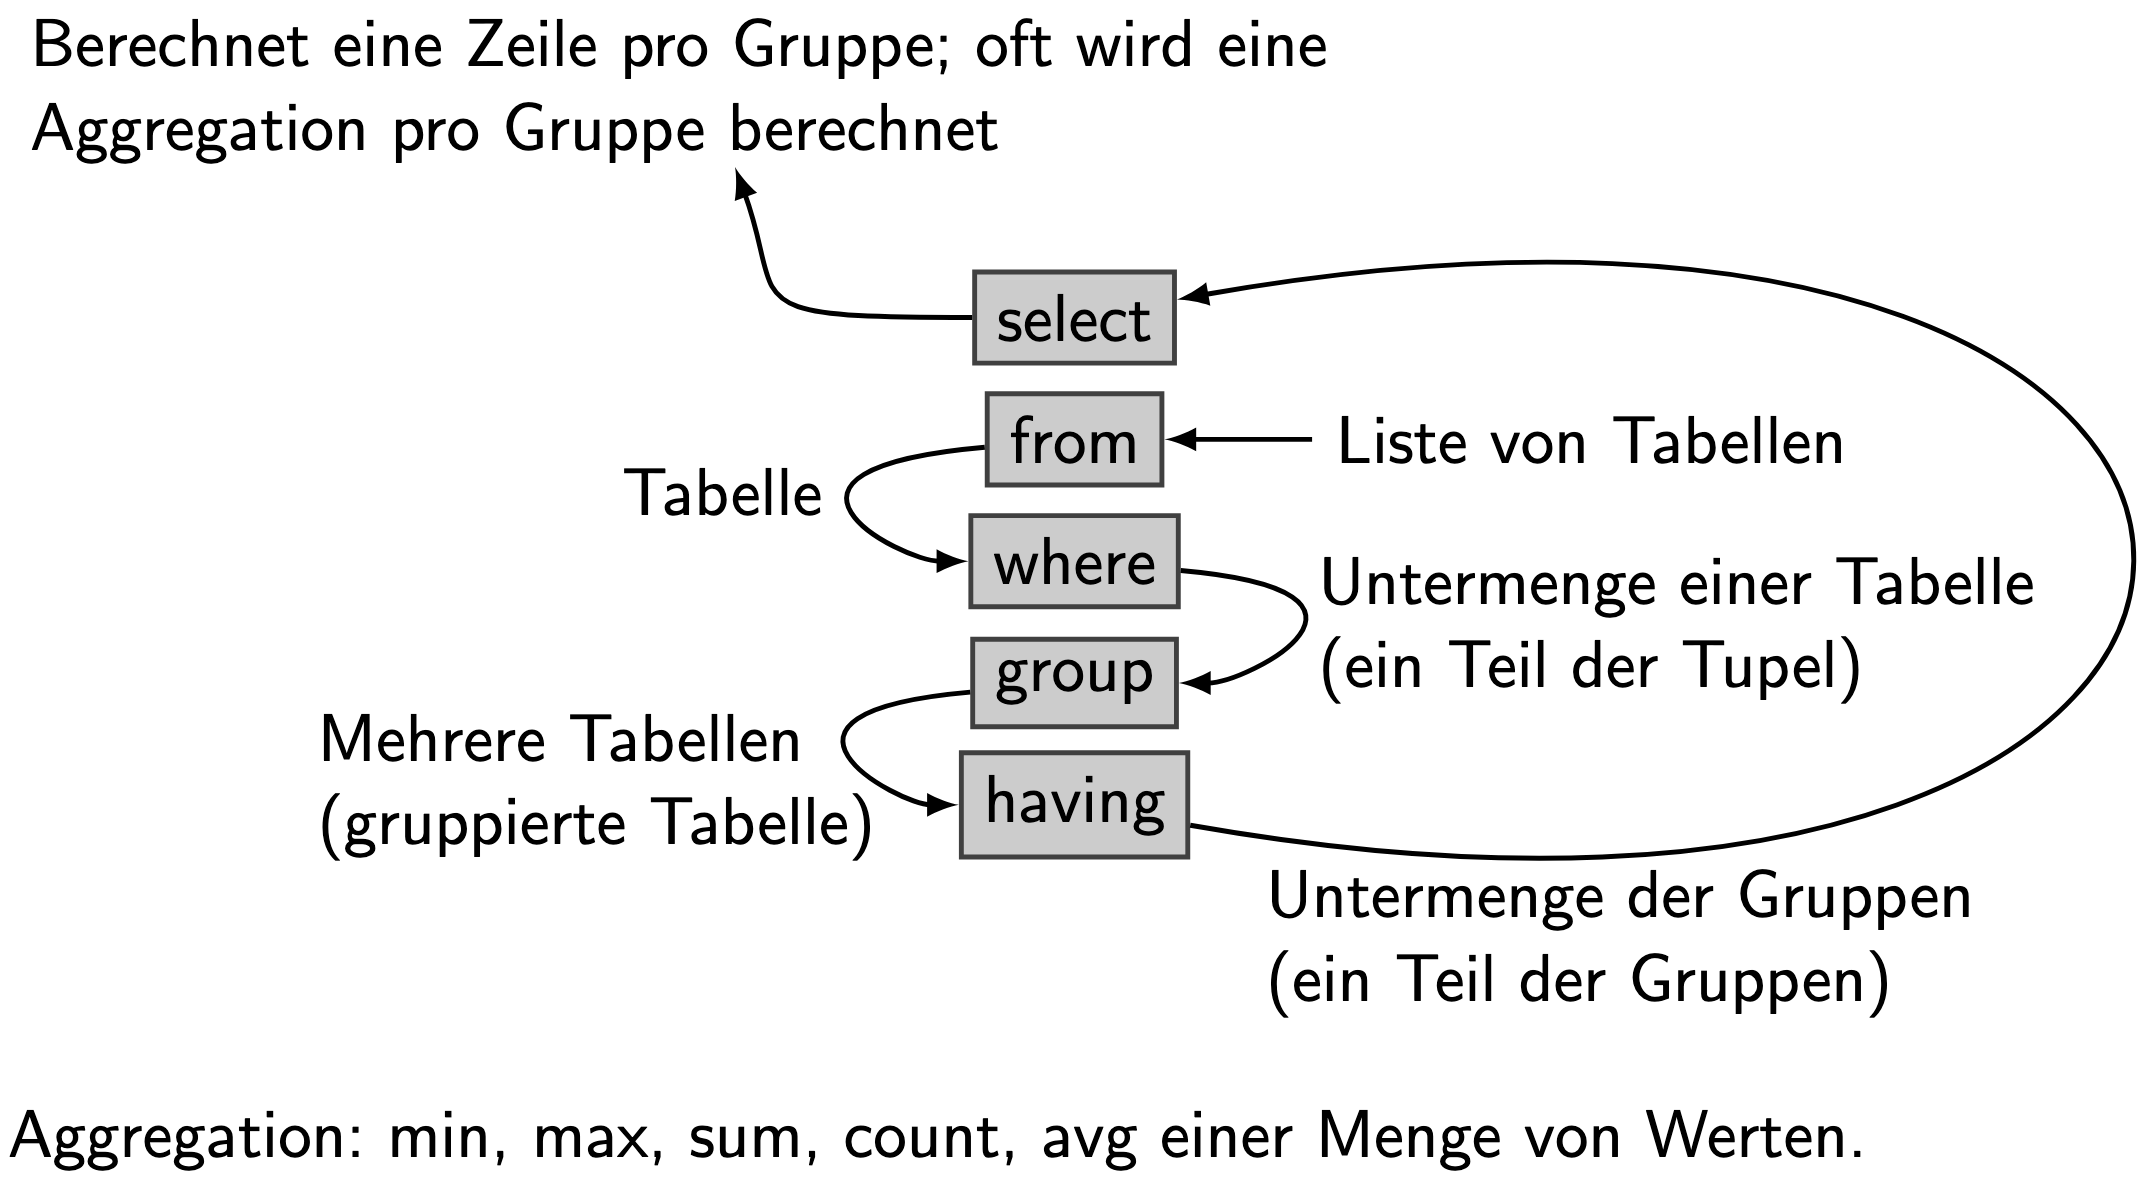
\includegraphics[scale=0.3]{Bilder/sql_flow.png}
 	\caption{Die Reihenfolge der Abarbeitung eines SQL Befehls}
 	\end{figure}
 	Anfragen in SQL haben eine spezifische Form. Die keywords \verb|select, from, where| oder \verb|group| sind eine Anfragespezifikation, welche mit \verb|union, except| oder \verb|intersect| verbunden werden können.
 	\subsubsection{Anfragen}
 	\paragraphlb{FROM}
 	Gibt alle Tabellen an die in der Anfrage involviert sind. Man kann Tabellen auch mittels \verb|as| Umbenennen um sie einfacher verwenden zu können, oder um Konflikte zu vermeiden.
 	\paragraphlb{WHERE}
 	Nimmt alle Tabellen aus \verb|from| und gleicht sie mit den Vorraussetzungen ab. Äquivalent zum Select $\sigma$. Gleich wie bei Select kann man verschiedene \verb|where| mit logischen Operatoren verknüpfen.
 	\paragraphlb{GROUP}
 	Partitioniert eine Tabelle in nicht überlappende Gruppen. Nimmt als Eingabe die Tabelle, welche durch \verb|where| produziert wurde.
 	\paragraphlb{HAVING}
 	Nimmt mittels \verb|group| gruppierte Gruppen und nimmt nur jene, welche die Anforderung erfüllen. Dabei wird die Entscheidung pro Gruppe gewählt und ausgewählt sobald mindestens ein Tupel die Anforderung erfüllt.
 	\paragraphlb{SELECT}
 	Spezifiziert weiter welche Resultate vorkommen sollen. Hierbei unterscheiden sich relationale Algebra und SQL, da SQL standardmäßig Duplikate im Ergebnis zulässt, weährend es in der relationalen Algebra durch die Verwendung von Sets nicht möglich ist. Man kann jedoch durch Verwendung des \verb|distinct| keywords spezifizieren, dass Duplikate verworfen werden sollen. \\
 	In \verb|select| kann man die bereits bekannten Aggregationsfunktionen verwenden und so etwa mit count() spezifizieren, dass man die Menge der erhaltenen Spalten wissen will. Der Stern \verb|*| steht dabei für alle möglichen. Wenn man also \verb|SELECT * FROM| angibt, will man alle Resultate haben. Gleichzeitig kann man diesen auch in Aggregationsfunktionen verwenden, wenn man also count(*) angibt, zählt dies alle Spalten, während count(A) nur die Spalten A zählt. 
 	\subsubsection{Mengenoperationen}
 	\begin{figure}[H]
 	\centering
  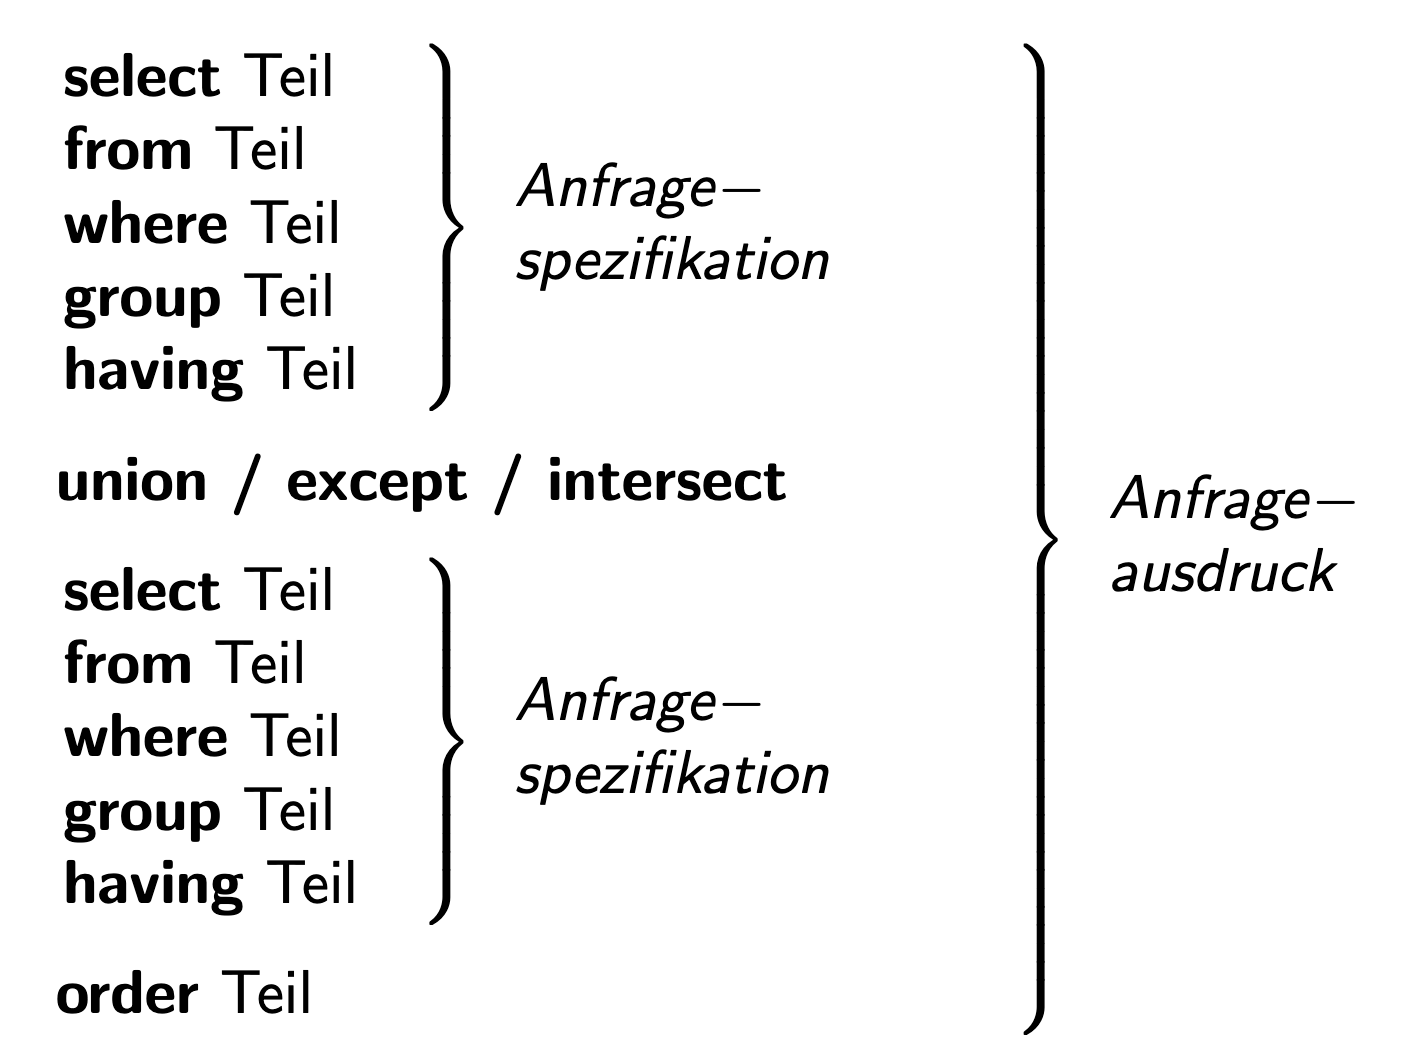
\includegraphics[scale=0.3]{Bilder/sql_union.png}
 	\caption{Verbindung von zwei SQL Queries}
 	\end{figure}
 	Gleich wie bei der relationalen Algebra, gibt es auch in SQL die Mengenoperationen. Diese sind \verb|union|, \verb|intersect| und \verb|except|. Da diese nun Mengenoperationen sind, werden Duplikate verworfen. Jedoch gibt es spezielle Operatoren, welche auch Duplikate auswählt. Die beiden verbundenen Mengen müssen wiederum \textit{Union Compatible} sein, setzen jedoch nicht mehr vorraus, dass die Attribute gleich heißen, sonder nur, dass sie den selben Typen haben. \\
 	Man muss jedoch beachten, dass bei solchen Operationen keine Namenskonflikte auftreten. Um diese zu vermeiden kann man eine Tabelle mit dem \verb|as| keyword umbenennen.
 	\subsubsection{null}
 	Da null eine gültige Belegung für alle Domänen sind, muss man auch mit diesem umgehen können. Da null für einen unbekannten Wert steht, darf die Überprüfung eines Attributes mit null keinen neuen Wert ergeben. Gleichzeitig ist auch die Abfrage ob null gleich null ist, Falsch (\verb|null=null -> False|). \\
 	SQL hat zusätzlich zu Wahr und Falsch noch einen dritten Wert, nämlich unknown. Jeder Vergleich mit null ergibt dabei unknown.
 	\begin{itemize}
 		\item{unknown \textit{oder} true = true}
 		\item{unknown \textit{oder} false = false}
 		\item{unknown \textit{oder} unknown = false}
 	\end{itemize}
 	\begin{itemize}
 		\item{true \textit{and} unknown = unknown}
 		\item{false \textit{and} unknown = false}
 		\item{unknown \textit{and} unknown = unknown}
 	\end{itemize}
 	\begin{itemize}
 		\item{\textit{not} unknown = unknown}
 	\end{itemize}
 	Wenn unknown Teil eines \verb|where| oder \verb|having| Prädikates ist, wird das als False behandelt. \\
 	\subsubsection{Ordnung}
 	Die Zeilen einer Tabelle sind standardmäßig nicht geordnet. Falls man das haben will, kann man das mit \verb|order by| verlangen. Wenn man nichts angibt wird es aufsteigend sortiert. Falls man es absteigend sortiert haben will, muss man \verb|desc| am Ende der Query angeben. Wenn man die aufsteigende Sortierung explizit angeben will, kann man natürlich auch \verb|asc| angeben.
	\subsection{Subqueries}
	Da SQL geschlossen ist, können \verb|select| Anweisungen geschachtelt werden. Dabei bezeichnet Unteranfrage einen Ausdruck, welcher innerhalb einer anderen Anfrage geschachtelt ist. \\
	In einem \verb|from| ist das die 'abgeleitete Tabelle', wodurch statt eines Tabellennamens eine SQL Anfrage gegeben sein kann. \\
	In einem \verb|where| ist es eine Mengenoperation, wobei man es als Argument innerhalb des Blocks verwenden kann. \\
	\begin{itemize}
		\item{exists, not exists}
		\item{in, not in}
		\item{some}
	\end{itemize}
	\subsubsection{Exists}
	Ist das Ergebnis der Subquery ungleich null: $exists(q) \iff q\ne \emptyset$ und $not\ exists(q) \iff q = \emptyset$. So kann man nachsehen, ob eine gewisse Menge überhaupt existiert, und nur dann eine Operation ausführt. \\
	\verb|select KName from Kontoinhaber as KI where exists (select * from Leasingnehmer as LN where KI.KName = LN.KName)| \\
	Beispiel: Definieren sie einen SQL Befehl, welcher den größten Wert in R mit einer geschachtelten Anfrage bestimmt (ohne Aggregationsfunktion.) \\
	\verb|-> SELECT DISTINCT A FROM R AS R1 WHERE NOT EXISTS (SELECT * FROM R AS R2 WHERE R2.A > R1.A)| Vergleicht jeweils einen Wert aus der Teilanfrage mit der äußeren Anfrage und 
	\subsubsection{In}
	\verb|In| ist wahr, wenn es ein Ergebnistupel gibt, das gleich ist wie a. Es können auch 100 sein, es macht jedoch keinen Unterschied. Gleichzeitig ist \verb|not in| wahr, wenn nicht zumindest ein Tupel gleich ist. Es ist zu beachten, dass bei einer subquery falsche Tupel nur eingeschränkt vorkommen. \\
	Zum Beispiel sind: \verb|SELECT A FROM R,S WHERE R.A = S.X| und \verb|SELECT A FROM R WHERE A IN (SELECT X FROM S)| \textbf{nicht} äquivalent, da der obere Ausdruck die Tabellen verbindet und so falsche Tupel erzeugt, welche danach eingegrenzt werden. Der untere hingegen vergleicht nur die Ergebnisse aus dem Subquery und schränkt somit nur weiter ein, anstatt zu kombinieren. \\
	\verb|SELECT KName FROM Leasingnehmer WHERE KName IN (SELECT KName FROM Leasingnehmer)|
	\subsubsection{some}
	\verb|Some| setzt vorraus, dass zumindest ein Tupel der Bedingung entspricht. Dabei kann man die Vorraussetzung entsprechend anpassen, sodass man stattdessen abfragt, ob zumindest eines der Tupel größer als 5 ist. \verb|5 < some -> true|. \\
	Man kann ein \verb|some| jedoch auch mit = abfragen, was dann überprüft ob zumindest einer der gesuchten Werte vorhanden ist. Umgekehrt überprüft $\ne$ ob zumindest ein Wert nicht dem gesuchten Wert entspricht. \\
	\verb|SELECT DISTINCT KNr FROM Konten, Filiale WHERE Konten.Betrag > Filiale.Umsatz AND Filiale.Name = 'Filiale 1'| kann somit auch als \\ 
	\verb|SELECT KNr FROM Konten WHERE Betrag > SOME (SELECT Umsatz FROM Filiale WHERE Name = 'Filiale 1')| angeschrieben werden. \\
	\verb|= some| und \verb|in| sind ihrer Anwendung äquivalent. Da beide bei ihrer Überprüfung nachsehen, ob zumindest ein Element existiert, kann man sie auch gleich verwenden. Das Gegenteil \verb|<> some| und \verb|not in| führt jedoch \textbf{nicht} zum gleichen Ergebnis. \verb|not in| überprüft ob der gesuchte Wert im Datensatz existiert während \verb|<> some| überprüft ob \textbf{kein anderer} als der Wert existiert (Was sehr selten der Fall ist.)
	\subsubsection{all}
	\verb|all| hat eine ähnliche Funktion wie \verb|some|, dabei muss jedoch nicht nur ein, sondern jedes Element der Vorraussetzung entsprechen. Gleichzeitig existiert wieder ein \verb|= all| und $\ne$\verb| all|, wobei \verb|= all| überprüft, ob alle Werte dem gesuchten Wert entsprechen und $\ne$\verb| all| überprüft ob kein Wert dem gesuchten entsprechen. \\ \\
	Man sollte beachten, dass \verb|(not) exists| statt jedem \verb|in|, \verb|any| oder \verb|all| Subquery verwendet werden kann. Einige SQL Implementationen konvertieren alle Befehle in \verb|exists| Befehle um.
	\subsection{DML}
	\subsubsection{Delete und Drop}
	Mit \verb|delete| und \verb|drop| kann man Tabellen und Zeilen löschen. Der Unterschied ist, dass \verb|delete| Zeilen der Tabelle löscht, dabei jedoch das Schema behält. \verb|Drop| hingegen löscht \textbf{alles} inklusive Schemadefinition, Indizes, usw. der Tabelle. \\
	\verb|DELETE FROM Konten WHERE FName = 'Filiale 1 -> Löscht alle Konten der Filiale 1| \\
	\verb|DELETE FROM Kredite WHERE KNr NOT IN (SELECT KNr FROM Kreditnehmer) -> Löscht alle Kredite ohne Kreditnehmer| 
	\subsubsection{Einfügen}
	Mit \verb|insert| fügt man Tupel ein. Nicht angegebene Werte werden, falls möglich, mit null oder dem als default festgelegten Wert aufgefüllt. \\
	\verb|INSERT INTO Kunden VALUES ('K-1234', 'Stettinger', 5000) -> Fügt neues Tupel zu Kunden hinzu.| \\
	Hier wurde nur die Tabelle, jedoch nicht die Spalten angegeben, wodurch es von rechts nach links befüllt wird. Man kann auch die Spalten explizit angeben, falls man dazwischen einen Wert auslassen will: \\
	\verb|INSERT INTO Kunden(Betrag, Name) VALUES ('5000, 'Stettinger)|
	\subsubsection{Update}
	Mit \verb|update| kann man bereits existierender Werte neu definieren. \\
	\verb|UPDATE Konten SET Guthaben = Guthaben * 1,06 WHERE Guthaben > 10000| \\
	\verb|                                         -> Erhöht das Guthaben aller Konten über 10000 um 6%|
	\section{View}
	Views werden verwendet um die Sicht von Benutzern einzuschränken. Das kann nützlich sein, wenn nicht alle Tabellen einer Datenbank einsehbar sein sollen. Man kann jedoch auch spezifizieren, dass nur Zugriff auf berechnete Tabellen ermöglicht werden und der Benutzer nicht weiß wie die Tabelle selbst aussieht. So kann man für spezifische Anwendungszwecke Views erstellen, welche danach für eine bestimmte Benutzergruppe ersichtlich wird. Indem man nur eine berechnete Tabelle zur Verfügung stellt, kann man die wahre Struktur der Datenbank verheimlichen, und so potentielle Angriffsflächen verringern. Zusätzlich dazu kann man in einem View abgeleitete anstatt der echten Werte angeben, und so eine komplett andere Tabelle zur Verfügung stellen. Ein bedeutend einfacherer Anwendungsfall ist, dass man in einer Tabelle, wenn sie angesehen wird, geheime Information nicht inkludiert wird. \\
	Einen View erstellt man mittels \verb|CREATE VIEW <V(A1, A2)> AS <Anfrage>|, wobei V der Name der Sicht ist, <Anfrage> ein gültiger Ausdruck, welcher eine Anzahl an Spalten liefert und $A_i$, was eine Anzahl an Spalten zeigt. \\
	Der Spaltenname kann optional sein, falls der Ausfrageausdruck eindeutig ist. Da V eine virtuelle Tabelle erstellt, kann man auch normale Anfragen darauf anwenden. Da die Tabelle nur virtuell existiert wird die Information als Metadaten in der Datenbank gespeichert. \\
	\verb|CREATE VIEW Alle_Kunden AS (SELECT FName, KName FROM Kontoinhaber, Konten WHERE Kontoinhaber.KNr = Konten.KNr)|
	\subsection{View Expansion}
	Bei der Auswertung des Views wird der Name des Views durch den entsprechenden Anfrageausdruck ersetzt.
	\subsection{Änderbarkeit}
	Ein View kann verändert werden, vorrausgesetzt die Umkehrabbildung kann die Basistabelle wiederherstellen. Das kann geschehen wenn:
	\begin{itemize}
		\item{distinct}
		\item{group by}
		\item{having}
		\item{SELECT enthält Spaltennamen mehrmals}
		\item{FROM enthält mehrere Views oder Tabellen}
	\end{itemize}
	\subsection{Temporärer View}
	Man kann auch temporäre Views erstellen, diese sind nur innerhalb des Anfrageausdrucks verfügbar. Einen temporären View definiert man mit \verb|with|.
	\section{Data Control Language (DCL)}
	SQL bietet zusätzlich noch eine Datenkontrollsprache, welche Zugriffsrechte einschränken kann. Das passiert mit den keywords \verb|grant| und \verb|revoke|. Zusätzlich kann man auch Festlegen wie viel CPU Zeit ein Benutzer jeweils bekommt.\\
	Man kann Zugriffsrechte entweder direkt an Personen vergeben oder Rollen definieren und diese vergeben. Größere Firmen vergeben sehr selten Zugrifssrechte an Person, da es bedeutend effizienter ist diese zentral als Rollen zu verwalten. 
	Man kann Zugriffsrechte auf verschiedenen Ebenen gewähren und entziehen.
	[TODO]
	System: tablespace
	Schema: Cluster, Index, Trigger, Datenbank
	Tabellen: create, alter, index, drop, select, delete, insert
	\\
	\subsection{grant}
	Mit \verb|grant| gewährt man Zugriffsrechte. Dabei können Zugriffsrechte nur von Benutzern vergeben werden, die diese Rechte selbst besitzen. \\
	\verb|GRANT <Liste von Zugriffsrechte> ON <Tabelle/View> TO <Liste von Benutzern>| \\
	\verb|                             -> Gewährt Benutzern Rechte innerhalb der Tabelle|
	\subsection{revoke}
	Mit \verb|revoke| entzieht man Rechte wieder. Dabei muss man beachten, dass man auch nur Rechte entziehen kann, welche man selbst besitzt. Zusätzlich kann es passieren, dass ein Benutzer weiter Rechte nach dem Entzug besitzt, da er die Rechte bereits von einem anderen Benutzer erhalten hat. Mann kann mit dem keyword \verb|all| auch alle Zugriffsrechte eines Benutzers entziehen.
	\verb|REVOKE <Liste von Zugriffsrechten> ON <Tabelle/View> TO <Liste von Benutzern>| \\
	\verb|                             -> Entzieht Benutzern Rechte innerhalb der Tabelle|
	\section{Datenbankzugriff}
	Die Schnittstelle eines Programms zu der Datenbank erlaubt das direkte Ansprechen der Datenbank über eine Programmiersprache. Einige solche Systeme sind: Embedded SQL, ODBC oder JDBC. \\
	Als Schnittstelle agiert hier ein Application Programming Interface (API). \\
	In Java wird normalerweise der Java Database Connectivity (JDBC) verwendet, welcher von Sun Microsystems entwickelt wurde und nach deren Übernahme von Oracle weiterverwaltet wird.
	\section{Richtlinien zum Datenbankentwurf}
	Bei dem Entwurf einer relationalen Datenbank ist das Hauptziel stets ein gutes und effektives Schema. Es kann sehr komplex sein eine passende Gruppierung seiner Daten zu erstellen. Das Hauptproblem dabei besteht die Definition einer 'guten' Datenbank, da dies meist von dem speziellen Anwendungsfall abhängt. Zur Klassifizierung gibt es die Datenbanknormalformen.
	\subsection{Anomalien}
	Anomalien sind Probleme, welche als Konsequenz eines spezifischen Schemas entstehen. Zum Beispiel, wenn man das Schema Projekt(\underline{SVN, PNr}, h, AName, PName, POrt) ansieht.
	\begin{itemize}
		\item{Updateanomalie}
		\begin{itemize}
			\item{Wenn der Projektort geändert wird, muss er für jeden Angestellten im Projekt geändert werden.}
		\end{itemize}
		\item{Einfügeanomalie}
		\begin{itemize}
			\item{Ein Projekt kann nicht angelegt werden, wenn es keine Angestellten hat, da es Teil des Primärschlüssels ist.}
		\end{itemize}
		\item{Löschanomalie}
		\begin{itemize}
			\item{Wenn ein Projekt gelöscht wird, werden auch alle Angestellten, welche an dem Projekt arbeiten gelöscht.}
		\end{itemize}
	\end{itemize}
	\subsubsection{Richtlinien für guten Entwurf}
	Es gibt vier Regeln um eine Datenbank so effektiv wie möglich zu gestalten:
	\begin{enumerate}
		\item{Jedes Tupel einer Relation sollte nur die Instanz einer Entität oder Beziehung darstellen.}
		\item{Update-, Lösch-, und Einfügeanomalien sollten vermieden werden.}
		\item{Relationen sollten so wenige NULL Werte wie möglich enthalten.}
		\begin{itemize}
			\item{Falls man relevante Daten hat, welche erst später eingefügt werden, sollte man diese in einer neuen Tabelle verpacken.}
			\item{In der Regel, sollte man so wenige Tabellen wie möglich, aber so viele wie nötig erstellen.}
		\end{itemize}
		\item{Durch einen natürlichen JOIN von Relationen sollten keine falschen Tupel erzeugt werden.}
	\end{enumerate}
	\subsection{Funktionale Abhängigkeiten (FD)}
	FDs werden zwischen Attributmengen einer Relatione gebildet. Y gilt als von X funktional abhängig wenn der Wert von X einen eindeutigen Wert von Y in der Relation vorgibt. Werte einer Tabelle sind beispielsweise voll funktional abhängig von dem Primärschlüssel. \\
	FDs definieren also eine EInschränkung auf das Schema (Und damit alle Instanzen von R) \\
	\verb|{SVN} -> {PNummer} -> SVN bestimmt Projektnummer| \\
	Da FDs auf dem Schema definiert sind, müssen sie auch für alle Instanzen gelten. Aus diesem Grund wird statt \{A, B\} nur AB (oder A, B) geschrieben $\to$ AB $\to$ CDE statt \{A, B\} $\to$ \{C, D, E\}. \\
	\begin{tabular}{| l | l | l |}
		\toprule
		X & Y & Z \\ \midrule
		1 & 1 & 3 \\
		2 & 1 & 1 \\
		3 & 2 & 2 \\
		4 & 1 & 1 \\
		\bottomrule
	\end{tabular} \\
	In dieser Tabelle gilt $Z\ \to\ X$ nicht, da mit 1 jeweils 2 und 4 abgebildet werden, jedoch $Z\ \to\ Y$ sehr wohl, da mit 1 jeweils nur 1 abgebildet wird
	\subsubsection{Superschlüssel und FD}
	Es mag bereits aufgefallen sein, dass Super- und Kandidatenschlüssel in ihrer Funktion sehr ähnlcih zur Funktionalen Abhängigkeiten sind. Ein Superschlüssel ist dann gegeben, wenn $K\to sch(R)$, also jeder Wert des Superschlüssels jede Spalte eindeutig zuweisen kann.
	\subsubsection{Armstrong-Axiome}
	Für eine Menge F aus Abhängigkeiten kann man auch zusätzliche Abhängigkeiten herleiten, welche immer gelten, solange die Abhängigkeiten in F gelten:
	\begin{itemize}
		\item{Reflexivität: $Y \subseteq X \vdash X\to Y$}
		\begin{itemize}
			\item{Wenn Y eine Teilmenge von X ist, dann enthält X, Y. X enthält Y bedeutet dadurch, dass Y funktional abhängig von X ist.}
		\end{itemize}
		\item{Verstärkung: $X \to Y \vdash XZ \to\ YZ$}
		\begin{itemize}
			\item{Das Hinzufügen einer Menge verändert nicht deren Funktionale Abhängigkeit}
		\end{itemize}
		\item{Transitivität: $X\to\ Y, Y\to\ Z \vdash X\to\ Z$}
		\begin{itemize}
			\item{Wenn X Y bestimmt und Y Z bestimmt, dann bestimmt X auch Z.}
		\end{itemize}
	\end{itemize}
	Diese Axiome sind korrekt und vollständig, also kann man alle anderen Regeln von diesen ableiten: \\
	$X\to Y, X\to W, WY\to Z, \vdash X\to Z$ \verb|-> Kann man aus diesen Abhängigkeiten, diese herleiten?| \\ \\
	$X\to Y\vdash XX\to XY=X\to XY$ \verb|Da man X -> Y zu XX -> XY verstärken kann, gilt auch X -> XY| \\
	$X\to W, \vdash XY\to WY$ \verb|X -> W wird zu XY -> WY verstärkt.| \\
	$X\to XY, XY\to WY \vdash X\to WY$ \verb|Da X -> XY und XY -> WY gilt, gilt auch X -> WY| \\
	$X\to WY, WY\to Z \vdash X\to Z$ \verb|Da X -> WY und WY -> Z gilt auch X -> Z|
	\subsubsection{Zusätzliche Inferenzregeln}
	Diese zusätzlichen Regeln kann man aus den anderen herleiten:
	\begin{enumerate}
		\item{Dekomposition - $X\to\ YZ \vdash X\to Y, X\to Z$}
		\begin{itemize}
			\item{Wenn X YZ bestimmt, bestimmt X auch Y und Z separat.}
		\end{itemize}
		\item{Vereinigung - $X\to Y,\ X\to\ Z \vdash X \to\ YZ$}
		\begin{itemize}
			\item{Wenn X sowohl Y als auch Z bestimmt, bestimmt X auch YZ}
		\end{itemize}
		\item{Pseudotransitivität - $X\to\ Y, WY\to\ Z \vdash WX\to\ Z$}
		\begin{itemize}
			\item{Wenn X Y bestimmt und Y Teil einer anderen Abhängigkeit ist, sind diese austauschbar.}
		\end{itemize}
	\end{enumerate}
	\subsubsection{Hülle}
	Eine Hülle $F^+$ ist die Menge F von FDs die von F hergeleitet werden können. Eine Hülle H(F, X) einer Menge von Attributen X bezüglich F ist die Menge aller Attribute, welche von X funktional abhängig sind. \\
	Hier werden die Armstrong Axiome relevant, da sowohl $F^+$ als auch H(F,X) durch Anwendung der Armstrong Axiome berechnet werden kann. \\
	Diesen kann man als Pseudocode wiedergeben. Dabei ist der Input die Menge F von FDs mit der Attributmenge X. Als Output soll die Attributhülle von X bezüglich F ausgegeben werden:
	\begin{verbatim}
	H(F,X)
	  Result:=X -> X bestimmt immer sich selbst
	  while (Result changes) do
	    foreach FD A -> B in F do -> Gehe alle potentiellen Funktionalen Abhängigkeiten durch
	      if A (Teilmenge) Result then Result := Result (Union) B -> Wenn A Teilmenge des Ergebnises ist, 
	  return Result                                                  füge es zur Endmenge hinzu
	\end{verbatim}
	Beispiel: \\
	$R[A, B, C, D]$ mit der Menge $F=\{AB\to D, B\to A, C\to B\}$ \verb|-> Was ist die Attributhülle von C?|
	\begin{verbatim}
	Erster Durchlauf: Ist C FD? Ja weil C immer mit sich selbst funktional Abhängig ist
	Zweiter Durchlauf: Ist B FD? Ja, weil C -> B -> Potentielle Menge hat sich geändert -> Neuer Durchlauf
	Dritter Durchlauf: Ist A FD? Ja, weil B -> A
	Vierter Durchlauf: Ist D FD? Ja, weil jetzt AB -> D
	H(F,X)={C,B,A,D}
	C-> ABCD
	\end{verbatim}
	Wenn man aus diesen FDs nun den besten Kandidatenschlüssel bestimmen will, sollte man sehen, welche rechts am seltensten vorkommt. Da C nie rechts steht, hat es auch das beste Potential für einen KS.
	\paragraphlb{Äquivalenz und Überdeckung}
	Zwei Mengen F und G sind genau dann äquivalent wenn:
	\begin{itemize}
		\item{Jede funktionale Abhängigkeit in F von G und in G von F hergleitet werden kann. (F ist eine Überdeckung von G / G ist eine Überdeckung von F)}
	\end{itemize}
	\paragraphlb{Äquivalenz und Membership}
	Bei dem Membership überprüft man, ob $X\to\ Y$ in $F^+$ ist. Man kann bestimmen, ob eine FD in einer Hülle ist, indem man überprüft, ob diese in der Hülle ist. That's it. \\
	Die Äquivalenz (Also das \verb|all| zum \verb|in|) zwischen F und G kann überprüft werden, indem jeweils überprüft wird, ob eine FD in beider Menge in der Hülle der anderen ist. \verb|-> Ist jede FD in F in G+? / Ist jede FD in G in F+?| \\
	\verb|                                                              Wenn ja, sind sie äquivalent.|
\end{document}